\begin{center}
	\LARGE
	Med hjælpemidler
\end{center}
\begin{opgavetekst}{Opgave 1}
	To linjer $l$ og $m$ er givet ved henholdsvis
	\begin{align*}
		l: \ 5x + 19y &= 12, \\
		m: \ 10x -10y &= 29.
	\end{align*}
\end{opgavetekst}
\begin{delopgave}{1}
	Orientér dig i Maple-filen \textit{To ligninger med to ubekendte} under forløbet \textit{Ligninger} på Teams og bestem derefter 
	skæringspunktet mellem $l$ og $m$. 
\end{delopgave}
\begin{delopgave}{2}
	Bestem løsningen til ligningssystemet
	\begin{align*}
		x + 2y + 3z &= 10,\\
		10x -5y + 3z &= 8, \\
		-2x + 9y -11z &= -3.
	\end{align*}
\end{delopgave}
\begin{opgavetekst}{Opgave 2}
	To polynomier $p$ og $q$ er givet ved
	\begin{align*}
		p(x) &= -2x^3 + 14x^2 + 8x - 100,\\
		q(x) &= -5x^3 - 13x^2 -10x + 68. 
	\end{align*}
\end{opgavetekst}
\begin{delopgave}{1}
	Orientér dig i Maple-filen \textit{Graftegning i Maple} under \textit{Vækst} på Teams og tegn graferne for $p$ og $q$ for $x \in [-8,3]$.
\end{delopgave}
\begin{delopgave}{2}
	Bestem koordinatsættet til skæringspunkterne for graferne til $p$ og $q$, og sammenlign dit resultat med 
	tegningen af graferne. 
\end{delopgave}

\newpage

\begin{opgavetekst}{Opgave 3}
	En funktion $f$ er givet ved
	\begin{align*}
		f(x) = b \cdot a^x
	\end{align*}
	og opfylder, at $f(2) = 5$ samt $f(4) = 12$
\end{opgavetekst}
\begin{delopgave}{1}
	Bestem tallene $b$ og $a$. 
\end{delopgave}
\begin{meretekst}
	En anden funktion $g$ er givet ved
	\begin{align*}
		g(x) = 1.2 \cdot x^d 
	\end{align*}
	og opfylder også, at $g(2) = 5$. 
\end{meretekst}
\begin{delopgave}{2}
	Bestem tallet $d$ og tegn grafen for $g$. 
\end{delopgave}
\begin{delopgave}{2}
	Orientér dig i Maple-filen \textit{Ligningsløsning på interval} under forløbet \textit{Ligninger} og bestem det andet skæringspunkt
	 mellem $f$ og $g$. 
\end{delopgave}

\begin{opgavetekst}{Opgave 4}
	\begin{center}
		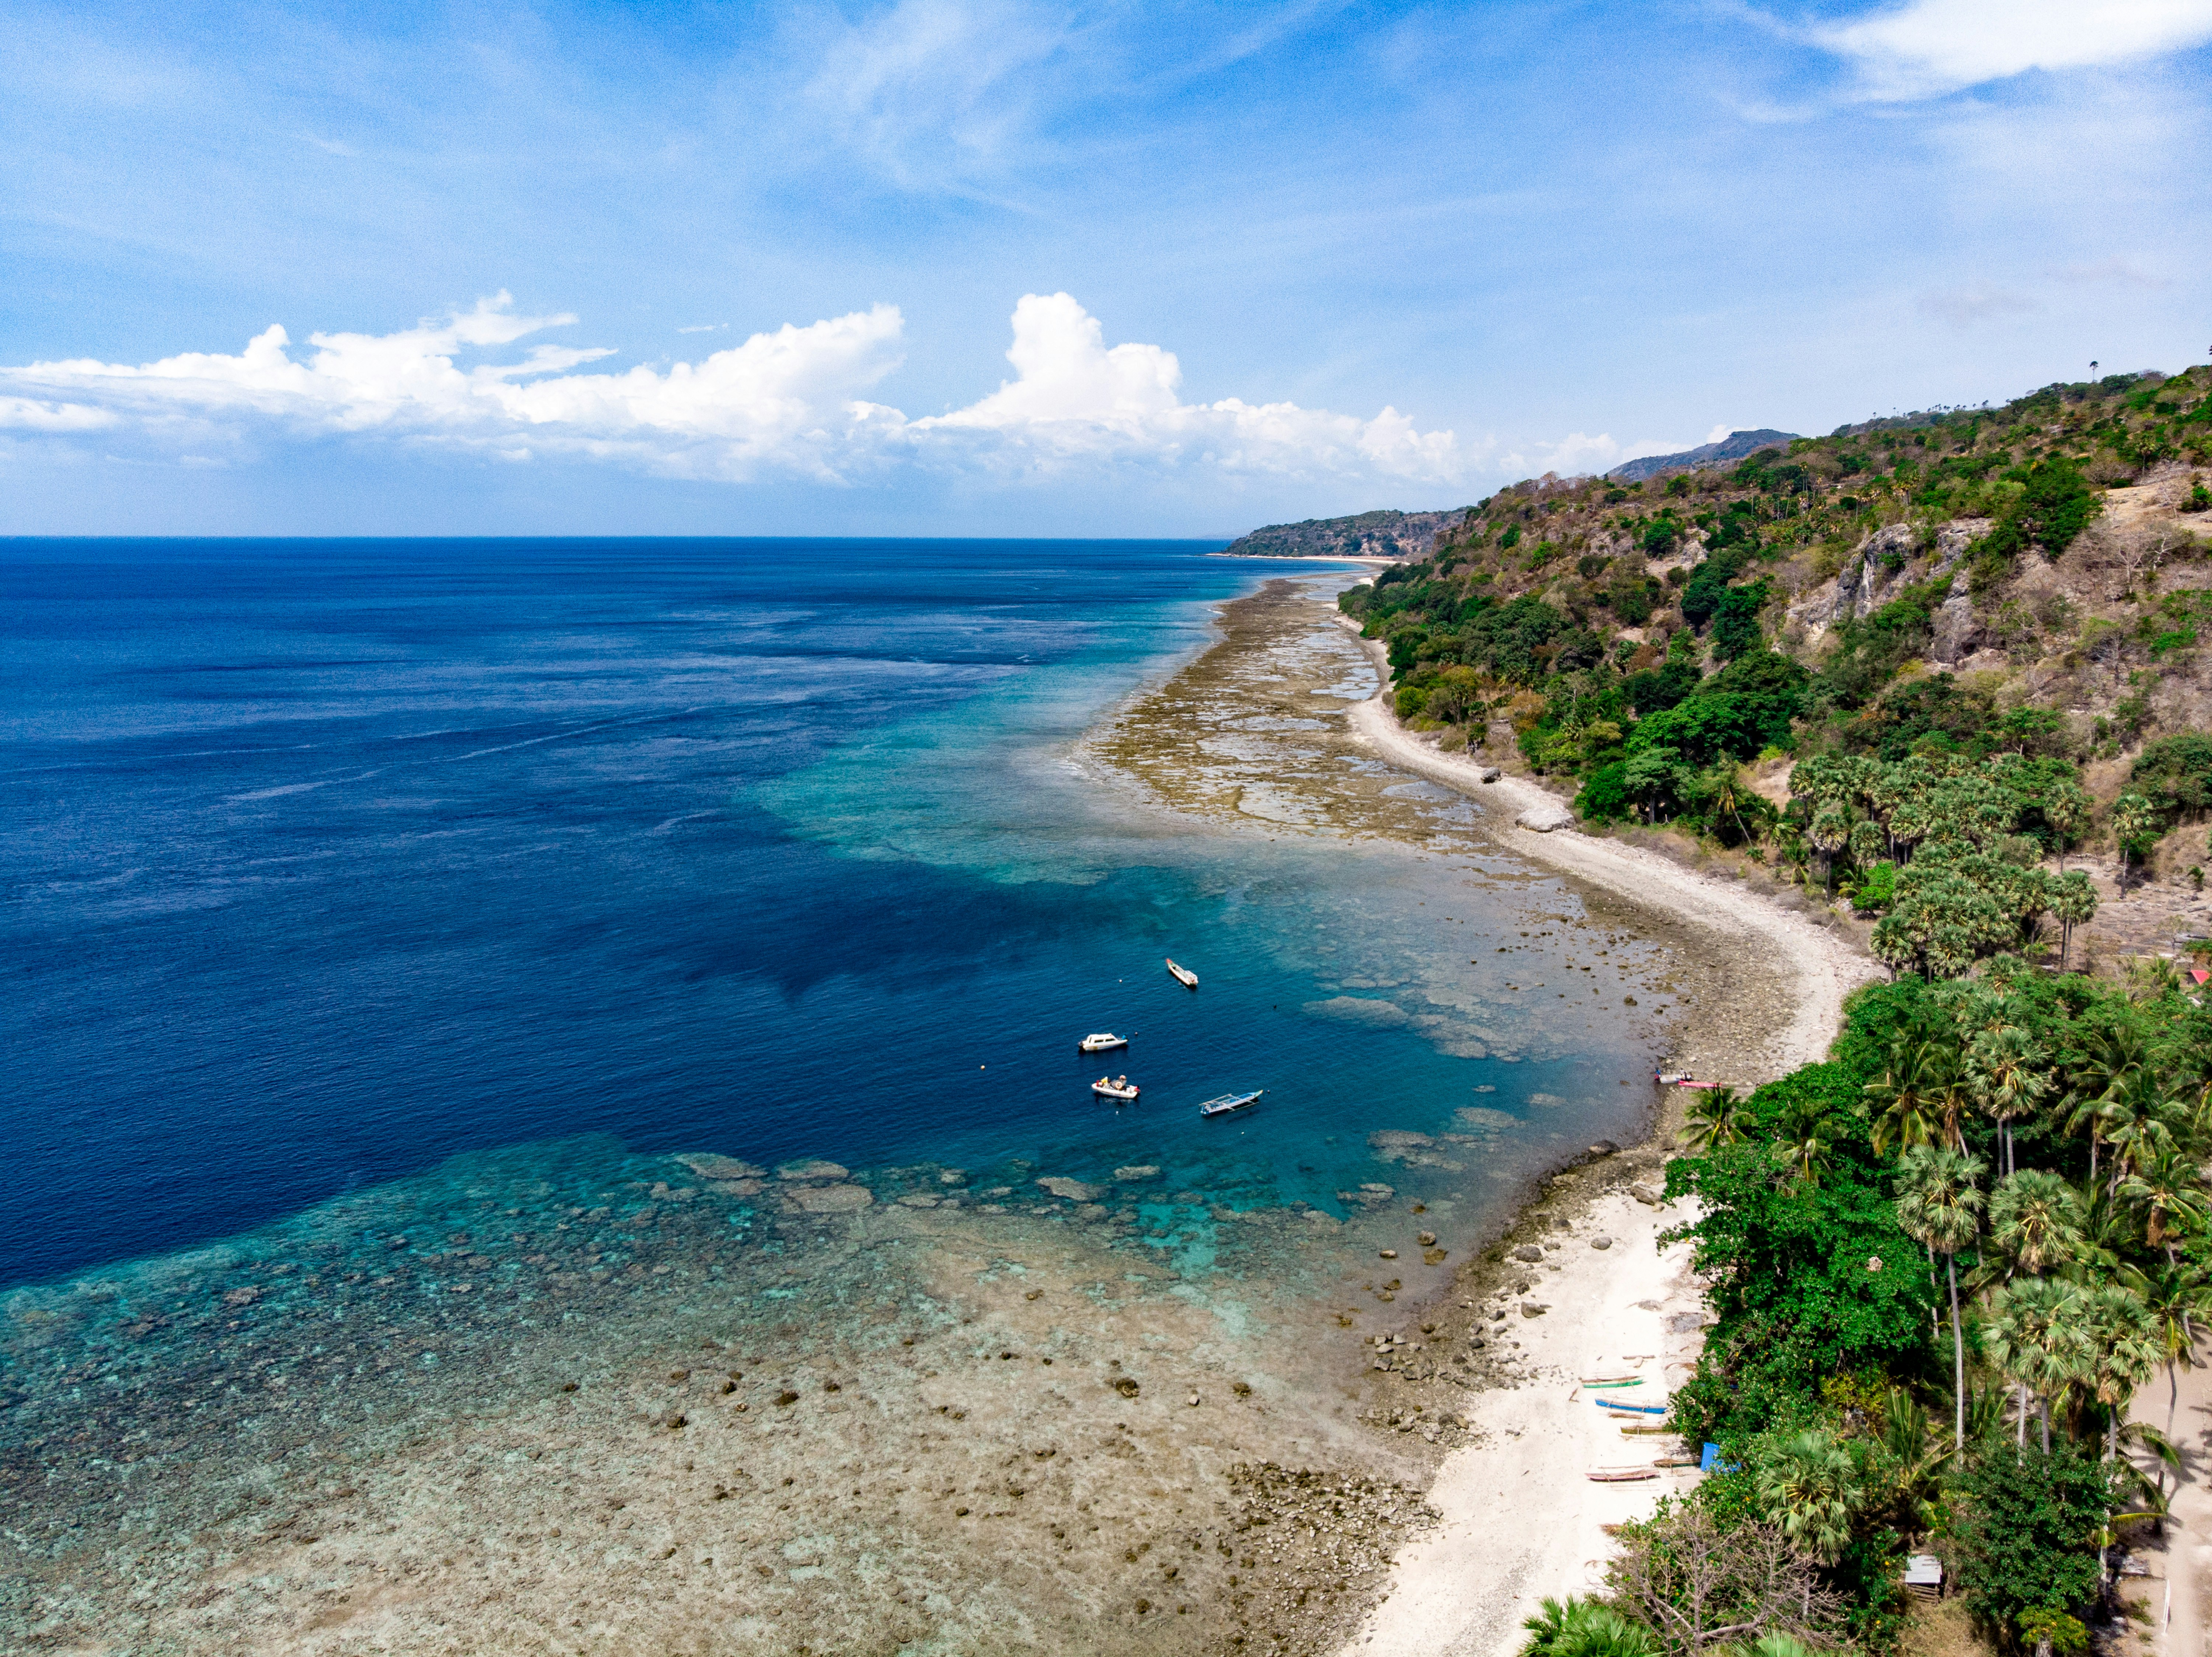
\includegraphics[width = 0.6\textwidth]{Billeder/oesttimor}
	\end{center}
	Bruttonationalproduktet i tidsperioden 1998-2023 for den tidligere portugisiske koloni Østtimor fremgår af \href{https://github.com/ChristianJLex/TeachingNotes/raw/master/2024-2025/Data%20og%20lign/BNPoesttimor.xlsx}{\color{blue!60}dette datasæt.}
	Det formodes, at den forløbne tid efter 1998 $t$ og BNP i Østtimor $f$ (i mia. USD) kan beskrives ved en sammenhæng af
	typen
	\begin{align*}
		f(t) = b\cdot a^t
	\end{align*}	 
\end{opgavetekst}
\begin{delopgave}{1}
	Orientér dig i filen \textit{Ændring af årstal} under \textit{Vækst} på Teams og bestem tallene $b$ og $a$.
\end{delopgave}
\begin{delopgave}{2}
	Giv en fortolkning af tallene $a$ og $b$. 
\end{delopgave}
\begin{delopgave}{3}
	Bestem det årstal, hvor Østtimor vil have et BNP på 40 mia ifølge modellen. 
\end{delopgave}
\newpage

\begin{opgavetekst}{Opgave 5}
	Et polynomium $p$ er givet ved
	\begin{align*}
		p(x) = 7x^5+2x^3-10x^2+5x+12
	\end{align*}
\end{opgavetekst}
\begin{delopgave}{1}
	Orientér dig i filen \textit{Rødder for polynomier} under \textit{Polynomier} på Teams og bestem rødderne for $p$.
\end{delopgave}